\documentclass[serif, aspectratio=169]{beamer}
\usepackage[T1]{fontenc} 
\usepackage{fourier}
\usepackage{hyperref}
\usepackage{latexsym,amsmath,xcolor,multicol,booktabs,calligra}
\usepackage{booktabs} % For better table formatting
\usepackage{graphicx,pstricks,listings,stackengine}
\usepackage{listings}
\usepackage{array} 
\usepackage{colortbl}

\author{Dr.Hajialiasgari}
\title{Machine Learning}
\institute{
    Tehran University \\
    Of\\
    Medical Science
}
\date{\small \today}
\usepackage{UoWstyle}

% Define custom colors and styles for listings
\definecolor{deepblue}{rgb}{0,0,0.5}
\definecolor{deepred}{RGB}{153,0,0}
\definecolor{deepgreen}{rgb}{0,0.5,0}
\definecolor{halfgray}{gray}{0.55}

\lstset{
    basicstyle=\ttfamily\small,
    keywordstyle=\bfseries\color{deepblue},
    emphstyle=\ttfamily\color{deepred},
    stringstyle=\color{deepgreen},
    numbers=left,
    numberstyle=\small\color{halfgray},
    rulesepcolor=\color{red!20!green!20!blue!20},
    frame=shadowbox,
}

\begin{document}

\begin{frame}
    \titlepage
    \vspace*{-0.6cm}
    \begin{figure}[htpb]
        \begin{center}
            \includegraphics[keepaspectratio, scale=0.05]{Tumsl-logo.png}
        \end{center}
    \end{figure}
\end{frame}

\begin{frame}    
\tableofcontents[sectionstyle=show, subsectionstyle=show/shaded/hide, subsubsectionstyle=show/shaded/hide]
\end{frame}

\section{Getting Started with \newline
Numpy and Pandas}
\section{NumPy}
\begin{frame}{What is NumPy?}
    \begin{itemize}
        \item NumPy is the fundamental package for scientific computing in Python.
        \item It is a Python library that provides a multidimensional array object, various derived objects,and an assortment of routines for fast operations on arrays, including mathematical, logical, shape manipulation, sorting, selecting, basic linear algebra , basic statical operations, random simulation and much more.
    \end{itemize}
\end{frame}

\begin{frame}{Application of NumPy}
    \begin{itemize}
        \item Mathematics
        \item Plotting
        \item Machine Learning
    \end{itemize}
\end{frame}

\begin{frame}{The Basics of NumPy}
    \begin{itemize}
       \item \texttt{\color{red}np.array()} - Create NumPy array
       \item \texttt{\color{red}ndim} - Returns dimension of the NumPy array
       \item \texttt{\color{red}shape} - Returns shape of the NumPy array
       \item \texttt{\color{red}dtype} - Returns data type of that NumPy array
       \item \texttt{\color{red}itemsize} - Returns size of that NumPy array in bytes
    \end{itemize}
\end{frame}

\begin{frame}{Concept of Slicing in NumPy}
    \begin{itemize}
       \item \texttt{\color{red}Array[row,:]} - Specific row and all columns
       \item \texttt{\color{red}Array[;,column]} - Specific columns and all rows
       \item \texttt{\color{red}Array[row,column]} - Specific row and specific column
    \end{itemize}
\end{frame}

\begin{frame}{Initializing NumPy Arrays}
    \begin{itemize}
       \item \texttt{\color{red}np.zeros()} - Create a array/matrix containing all '0's element.
       \item \texttt{\color{red}np.ones()} - Create a arraye/matrix containing all '1's element.
       \item \texttt{\color{red}np.ranodm.full()} - Create a array/matrix eith containing all elements a specified value.
       \item \texttt{\color{red}np.ranodm.rand()} - Create a array/matrix containing all elements decimal valued randomly.
       \item \texttt{\color{red}np.ranodm.randint()} - Create a array/matrix containing all elements integer valued randomly.
       \item \texttt{\color{red}astype()} - Change the datatype of the data
    \end{itemize}
\end{frame}

\begin{frame}{Reorganizing Arrays}
    \begin{itemize}
       \item \texttt{\color{red}Reshape()} - Change the shape of array/matrix
       \item \texttt{\color{red}Vstack()} - Stack arrays in sequence vertically (row wise).
       \item \texttt{\color{red}Hstack()} - Stack arrays in sequence horizontally (column wise).
    \end{itemize}
\end{frame}

\section{Pandas}
\begin{frame}{What is Pandas?}
    \begin{itemize}
        \item Pandas is a Python library used for working with datasets.
        \item It has functions for analyzing, cleaning, and manipulating data.
    \end{itemize}
\end{frame}

\begin{frame}{What is Dataframe?}
    \begin{itemize}
        \item A Pandas DataFrame is a 2 dimensional data structure, like a 2 dimensional array , or a table with rows and columns.
    \end{itemize}
\end{frame}

\begin{frame}{Loading DataFrame}
    \centering
    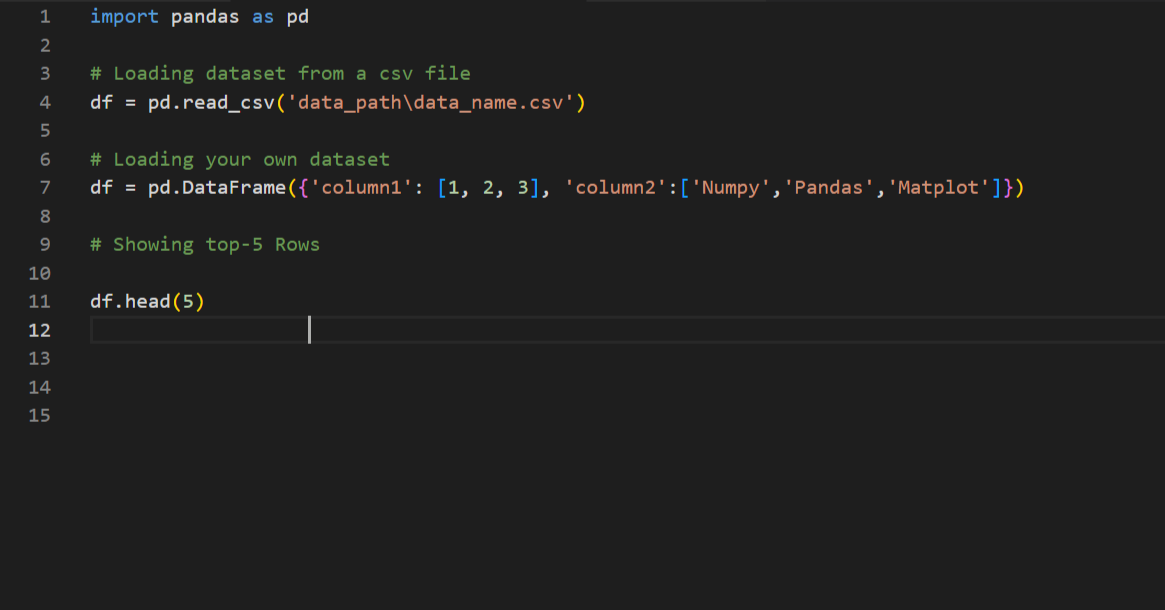
\includegraphics[width=0.7\textwidth, height=0.7\textheight]{Loadingdata.png}
\end{frame}

\begin{frame}{Extract Data from Dataframe}
    \begin{itemize}
        \item \texttt{\color{red}df.head()}
        \item \texttt{\color{red}df.tail()}
        \item \texttt{\color{red}df.columns}
        \item \texttt{\color{red}df.index}
        \item \texttt{\color{red}df.info()}
        \item \texttt{\color{red}df.size}
        \item \texttt{\color{red}df.describe()}
        \item \texttt{\color{red}df.shape}
        \item \texttt{\color{red}df.dtype}
    \end{itemize}
\end{frame}

\begin{frame}{Value at Specific Cell}
    \begin{itemize}
        \item \texttt{\color{red}df.at[row\_index,column\_name]}
        \item \texttt{\color{red}df.iat[row\_index,column\_index}
    \end{itemize}
\end{frame}

\begin{frame}{Fetch a Record}
    \begin{itemize}
        \item \texttt{\color{red}df.loc[rows]} - row can be integer or non-int value
        \item \texttt{\color{red}df.iloc[rows]} - row must be integer
    \end{itemize}
\end{frame}

\begin{frame}{Find, Remove Null}
    \begin{itemize}
        \item \texttt{\color{red}isna()}
        \item \texttt{\color{red}fillna()}
        \item \texttt{\color{red}Dropna(inplace=True)}
    \end{itemize}
\end{frame}

\begin{frame}{Properties}
    \begin{itemize}
        \item \texttt{\color{red}max()}
        \item \texttt{\color{red}min()}
        \item \texttt{\color{red}mean()}
        \item \texttt{\color{red}unique()}
        \item \texttt{\color{red}nunique()}
        \item \texttt{\color{red}value\_counts()}
    \end{itemize}
\end{frame}

\begin{frame}{Set Operation Using Concat Method}
    \begin{itemize}
        \item \texttt{\color{red}pd.concat([df1,df2])}
        \item \texttt{\color{red}df.append()}
    \end{itemize}
\end{frame}

\begin{frame}
    \begin{center}
        {\Huge\ End of NumPy and Pandas}
    \end{center}
\end{frame}

\end{document}

